\documentclass{article}
\usepackage{graphicx} % Required for inserting images

\usepackage{setspace}

\usepackage{amsmath}
\usepackage{color}

\usepackage{amsthm}
\usepackage{bm}

\usepackage{indentfirst}
\setlength{\parindent}{2em}  % 用于首行缩进

\newcommand{\Z}{\mathbf{Z}}
\newcommand{\D}{\bm{\Delta}}
\newcommand{\A}{\mathbf{A}}


\newtheorem{lemma}{\hspace{2em}Lemma}
\newtheorem{proposition}{\hspace{2em}Proposition}
\newtheorem{example}{Example}

\usepackage{geometry}
\geometry{a4paper,left=1in,right=1in,top =1in, bottom = 1in}
\setstretch{1.5}   %  改变行间距

\title{Appointment Scheduling with Restricted People}

% \author{Discount}

\date{}
\begin{document}

\maketitle

\section{Preliminary Study}

The service time for customer $i$, $\xi_{i}$, stochastic with a mean of $\mu_{i}$ and a standard deviation of $\sigma_{i}$. The service times are mutually independent.
For each customer $i = 1, \ldots, n$, we use $A_{i}$ to denote the appointment time, $S_{i} = \max\{A_{i}, S_{i-1} + \xi_{i-1}\}$ denote the actual starting time of service. We assume that the customers will arrive at the appointed time. Especially, $A_{1} = S_{1} = 0$.

The waiting time for customer $i$ is $S_{i} - A_{i}$, the total waiting time is $\sum_{i=2}^n \alpha_i \left(S_i-A_i\right)$, where $\alpha_i$ is the weight for customer $i$. The overtime is $(S_{n} +\xi_{n} - T)^{+}$ and the total idle time is $\sum_{i=1}^{n-1}[S_{i+1} - (S_{i} + \xi_{i})] = S_{n} - \sum_{i=1}^{n-1} \xi_{i}$.


\textcolor{red}{In the scenario with at least 2 customers overlapping in the waiting room, we can calculate the overlapping time. Let $t_{ij}$ denote the overlapping time between two customers $i$ and $j$. Then, $t_{i,j} = (S_{i} - A_{j})^{+}$}, indicating there are at least $(j-i+1)$ customers waiting.

The duration when there are only $(j-i+1)$ people from customer $i$ to customer $j$ are waiting is $t_{i,j} - t_{i,j+1}$, $i =2, \ldots, n-1, j \geq i$.

%  customer $i$ will arrive at $A_{i}$ but start service at $S_{i}$.

\textcolor{red}{Total overlapping time: $\sum_{i=2}^{n-1} \sum_{j=i}^{n-1} \gamma_{i,j} (t_{i,j} - t_{i,j+1})$}

Problem to minimize the total time cost:

\begin{equation}
    \begin{aligned}
        \min_{\mathbf{A}} \quad & E_{\xi}\left[\left(S_n-\sum_{i=1}^{n-1} \xi_i\right)+ \sum_{i=2}^{n-1} \sum_{j=i}^{n-1} \gamma_{i,j} (t_{i,j} - t_{i,j+1}) + \beta(S_{n} +\xi_{n} - T)^{+} \right] \\
        \mbox{s.t.} \quad & S_{i} = \max\{A_{i}, S_{i-1} + \xi_{i-1}\} \\
        & S_{1} = 0
    \end{aligned}
\end{equation}

To minimize the makespan:

\begin{equation}
    \begin{aligned}
        \min_{\mathbf{A}} \quad & E_{\xi}\left(S_n + \xi_{n}\right) \\
        \mbox{s.t.} \quad & E_{\xi}\left( t_{i,j} - t_{i,j+1} \right) \leq L_{ij}, i =2, \ldots, n-1, j \geq i
    \end{aligned}
\end{equation}

$L_{ij}$ indicates constraint on the duration of $(j-i+1)$ people waiting.


\section{Model}
We redefine the scheduling problem using the following notation. Let $\D = (\Delta_1, \ldots, \Delta_n)$ denote the \textbf{appointment intervals}, where $\Delta_{i}$ is the time allocated between the start of customer $i$ and customer $i+1$. Let $\A = (A_1, \ldots, A_n)$ represent the \textbf{scheduled appointment times}, with $A_{i} = \sum_{k=1}^{i-1} \Delta_{k}$ (assuming $A_{1}=0$). Let $\Z = (Z_1, \ldots, Z_n)$ be the \textbf{random service durations}, where $Z_{i}$ is the stochastic service time for customer $i$.

The waiting time for customer $i$ is recursively defined as:
\begin{align*}
  W_{i}(\Z_{i-1}, \D_{i-1}) &= [A_{i-1} + W_{i-1}(\Z_{i-2}, \D_{i-2}) + Z_{i-1} -A_{i}]^{+} \\
    & = [W_{i-1}(\Z_{i-2}, \D_{i-2}) + Z_{i-1} - \Delta_{i-1}]^{+},
\end{align*}
where $[*]^{+} = \max(*, 0)$. $W_{1}(\Z_{0}, \D_{0}) = 0$.

Let $W_{ij}$ denote the \textbf{simultaneous waiting duration} for customers $i$ through $j$, meaning the length of time during which all customers from $i$ to $j$ are simultaneously waiting. This can be expressed recursively as: $W_{i, j}(\Z_{i-1}, \D_{j-1}) = [W_{i-1}(\Z_{i-2}, \D_{i-2}) + Z_{i-1} - \sum_{k =i-1}^{j-1} \Delta_{k}]^{+}$, where $W_{i} \equiv W_{i,i}$ is the individual waiting time for customer $i$. $W_{ij}$ captures the time window where customers $i$ to $j$ all experience waiting simultaneously due to delays from earlier customers (1 to $i-1$) and insufficient buffer times.


The finish time for customer $i$ is $T_{i}(\Z_{i}, \D_{i-1}) = A_{i} + W_{i}(\Z_{i-1}, \D_{i-1}) + Z_{i}$. We aim to minimize the total schedule span, i.e., $T_{n}$, subject to constraints on individual and group waiting times.

The formulation of the problem can be expressed as follows

\begin{equation}\label{joint_waiting}
    \begin{aligned}
        \min \quad & E \left[T_n(\Z_{n}, \D_{n-1}) \right] \\
        \mbox{s.t.} \quad & E\left[W_{i,j}(\Z_{i-1}, \D_{j-1}) \right] \leq w_{ij}, i =2, \ldots, n-1, j \geq i
    \end{aligned}
\end{equation}


In this setting, $w_{ij}$ is related with the number of customers from $i$ to $j$, i.e., $j-i +1$. We can use $w_{k}$ to indicate the upper limit on the time when there are $k$ customers waiting.

$T_{n}(\Z_{n}, \D_{n-1}) = A_{n} + W_{n}(\Z_{n-1}, \D_{n-1}) + Z_{n}$.

\begin{lemma}
For any given realization of $\Z_{n}$, $T_n(\Z_{n}, \D_{n-1})$ becomes shorter when some customer is scheduled to arrive earlier while the schedule for others remain unchanged.
\end{lemma}

The optimal schedule can be obtained by minimizing $\Delta_{i}$.

When $i =1$, the first customer doesn't need to wait.

When $i =2$, only one constraint $E\left[W_{1}(\Z_{0}, \D_{0}) + Z_{1}- \Delta_{1} \right]^{+} \leq w_{1}$ is applied, then $\D_{1}^{*}$ can be obtained.

When $i =3$, there are two constraints on the waiting time of the third customer.

$E\left[W_{2}(\Z_{1}, \D_{1}^{*}) + Z_{2} - \Delta_{2}\right]^{+} \leq w_{1}$.

$E\left[W_{1}(\Z_{0}, \D_{0}) + Z_{1} - \Delta_{1}^{*} - \Delta_{2}\right]^{+} \leq w_{2}$.

When $i =n$, there are $(n-1)$ constraints.

\begin{proposition}
    By solving the above problems sequentially, the optimal schedule can be obtained.
\end{proposition}

Then we analyze these problems. The function on the left-hand side is decreasing in the variable $\Delta_{i}$.

When $\Delta_{1} = 0$, $E\left[W_{1}(\Z_{0}, \D_{0}) + Z_{1}- \Delta_{1} \right]^{+} = E\left[Z_{1}\right]^{+}$. If $E\left[Z_{1}\right]^{+} \leq w_{1}$, $\Delta_{1}^{*} = 0$; if $E\left[Z_{1}\right]^{+} > w_{1}$, $E\left[Z_{1}- \Delta_{1}^{*} \right]^{+} = w_1$.

If $Z_{i}$ follows from the exponential distribution with rate $\lambda$, $E\left[Z_{1}- \Delta_{1} \right]^{+} = \frac{1}{\lambda} e^{-\lambda \Delta_{1}}$, then

\begin{equation*}
	\Delta_{1}^{*} = \begin{cases}
	-\frac{\ln (\lambda w_{1})}{\lambda}, & \text{if}~ \lambda w_{1} < 1 \\
	0, & \text{if}~ \lambda w_{1} \geq 1	
	\end{cases}
\end{equation*}

% The optimal schedule for \eqref{joint_waiting} is feasible for \eqref{only_waiting} because the feasible region of \eqref{joint_waiting} is smaller than that of \eqref{only_waiting}.

% \begin{equation}\label{only_waiting}
%     \begin{aligned}
%         \min \quad & E \left[T_n(\Z_{n}, \D_{n-1}) \right] \\
%         \mbox{s.t.} \quad & E\left[W_{i,j}(\Z_{i-1}, \D_{j-1})-W_{i,j+1}(\Z_{i-1}, \D_{j}) \right] \leq w_{ij}, i =2, \ldots, n-1, j \geq i
%     \end{aligned}
% \end{equation}


% Surgical Scheduling with Constrained customer Waiting Times
% Appointment Scheduling Under a Service-Level Constraint


\newpage

\section{Literature}
% https://www.qmatic.com/blog/minimize-clinic-waiting-times-to-avoid-virus-spread

1. Possible traits: heterogeneous customers, no-show, lateness, walk-in

Different models: objective: minimize the total cost, minimize the makespan (the departure time of the last customer).

% Two possible options: the time of several people waiting, what if it is not makespan

Traditional Appointment Scheduling Model.

1. with overbooking and no-shows (partial punctuality)

- discrete n time slots.

- minimize the waiting cost, idle time and overtime costs.

- analyze three components seperately


2. Under a service-level constraint (waiting time threshold)

- makespan

- the optimal schedule can be obtained sequentially.


% \section{Deterministic Situation}
% % For the $k$th customer, arriving at $(k-1)t$, 

% % 我们考虑现有的 appointment scheduling 中 waiting time

% Suppose there are $n$ customers to be scheduled. If the hard constraint-that certain individuals cannot be in the waiting room simultaneously-cannot be satisfied, the number of customers to be scheduled must be reduced until a feasible schedule is achieved.

% Each customer $i$ has a service time $Z_{i} \in [\underline{Z}_{i}, \overline{Z}_{i}]$. The goal is to maximize the number of scheduled customers $n$. The appointment time of the last customer does not exceed a given deadline $\overline{T}$. The number of simultaneous waiting customers, $S(t)$, never exceeds the capacity $N$ at any time $t$.

% This yields the following deterministic optimization problem:

% \begin{equation}\label{deterministic_model}
%     \begin{aligned}
%         \max \quad & n \\
%         \mbox{s.t.} \quad & W_{i}(\Z_{i-1}, \D_{i-1}) = [W_{i-1}(\Z_{i-2}, \D_{i-2}) + Z_{i-1} - \Delta_{i-1}]^{+}  \\
%         & S(t) \leq N, \forall t  \in [0, \overline{T}] \\
%         & A_{n} \leq \overline{T}
%     \end{aligned}
% \end{equation}


% To obtain the number of simultaneous waiting customers, we define $j^{*}(i)$ as the largest index $j$ satisfying: 
% $$(\overline{Z}_{i-1}- \sum_{i-1}^{j-1} \Delta_{k})> 0, i =2, \ldots, n$$ 
% where $\Delta_{k}$ represents the appointment interval for customer $k$. The number of simultaneous waiting customers can be obtained by $j^{*}(i) -i +1$. Given a fixed schedule $\D$, the maximum $j^{*}$ can be computed explicitly.


% When all customers are assigned their maximum service time ($Z_{i} = \overline{Z}_{i}$), the schedule that maximizes the number of customers $n$ is obtained by solving:

% $$n^{*} = \max\left\{n\bigg|\sum_{i=1}^{n} \overline{Z}_{i} \leq \overline{T}\right\} + N +1,$$ where $\overline{T}$ is the deadline and $N$ is the waiting room capacity.

% \begin{example}
%     $Z_{i} \in [20, 40]$ for each $i$. $\overline{T} =120$. $N =2$. $n^{*} = 3 + 2 +1$. The optimal schedule is $A_{1} = 0$, $A_2 = 40$, $A_3 = 80$, $A_4 =A_5 = A_6 = 120$.
% \end{example}

% The counterpart (dual) problem aims to minimize the schedule time $A_n$ of the last customer, given a fixed number of customers $n$, while respecting the waiting area capacity constraint. The optimization problem is formulated as:

% \begin{equation}
%     \begin{aligned}
%         \min \quad & A_{n} \\
%         \mbox{s.t.} \quad & W_{i}(\Z_{i-1}, \D_{i-1}) = [W_{i-1}(\Z_{i-2}, \D_{i-2}) + Z_{i-1} - \Delta_{i-1}]^{+} \\
%         & S(t) \leq N, \forall t \in [0, A_n]
%     \end{aligned}
% \end{equation}


% \begin{example}
%     $n = 6$. $Z_{i} \in [20, 40]$ for each $i$. $N =2$. The optimal schedule is $A_{1} = 0$, $A_2 = 40$, $A_3 = 80$, $A_4 =A_5 = A_6 = 120$.
% \end{example}

% For any given realization of $\Z_n$, an optimal schedule is $A_1 = 0$, $A_i = \sum_{k=1}^{i-1} Z_k, 2 \leq i \leq n-N$, $A_{n-N+1} = \ldots = A_{n} = \overline{T}$.


% \section{Stochastic Situation}
% The soft constraint can be set as the expected number of simultaneous waiting people does not exceed certain number. 

% Or the probability of the largest number of simultaneous waiting people is less than a threshold.

% \begin{equation}\label{stochastic_model}
%     \begin{aligned}
%         \max \quad & n \\
%         \mbox{s.t.} \quad & E[S(t)] \leq N, \forall t \\
%         & A_{n} \leq \overline{T}
%     \end{aligned}
% \end{equation}

% \begin{equation}\label{stochastic}
%     \begin{aligned}
%         \min \quad & E \left[T_n(\Z_{n}, \D_{n-1}) \right] \\
%         \mbox{s.t.} \quad & E\left[S(t) \right] \leq N, \forall t
%     \end{aligned}
% \end{equation}

% The constraint $E\left[S(t) \right] \leq N, \forall t$ is equivalent to $E\left[S(A(i)) \right] \leq N, i=2,\ldots, n$.

% $S(A(i)) = \max\{j|W_{i-1} + Z_{i-1}-\sum_{i-1}^{j-1} \Delta_{k} >0\} - i + 1$.


% $T_{i}(\Z_{i}, \D_{i-1}) = \sum_{k=1}^{i-1} \Delta_{k} + W_{i}(\Z_{i-1}, \D_{i-1}) + Z_{i}$

% $W_{i}(\Z_{i-1}, \D_{i-1}) = [W_{i-1}(\Z_{i-2}, \D_{i-2}) + Z_{i-1} - \Delta_{i-1}]^{+}$

% If the constraint is hard, for each $i$, we have $\max\{j|W_{i-1} + Z_{i-1}-\sum_{i-1}^{j-1} \Delta_{k} >0\} - i + 1 \leq N$. The constraints can be converted to $Z_{i-1} + W_{i-1} \leq \sum_{i-1}^{N-2+i} \Delta_{k}, i =2 \ldots, n$.


\section{Some Measures}
Priority-Based Waiting Time Control: The waiting time for emergency patients is less than 15 minutes. No longer to serve conventional patients when the number of waiting patients is no less than 3. 
% 按病情优先级分级限制等待时间,

% 紧急患者:等待时间≤15分钟;

% 常规患者:若当前等待人数≥3人,自动分配至下一时段。

% 根据实时等待人数调整优先级阈值(如3人等待时,仅接收急诊患者)

% 新患者自动转入“快速通道”(等待时间承诺≤10分钟)

Time Slot-Based Waiting Time Control: fixed interval, adjust schedule interval according to the congestion, dynamically extend the schedule interval or shut down according to real-time data.

% 固定间隔, 动态调整时段长度(根据拥挤程度,调整固定间隔), new research: 当系统检测到未来某时段预约超额时,自动关闭该时段或延长间隔。

% 2. 存在 n 人时,但是可以 rescheduling, 用短信等方式通知预约人延后的信息

% 上网查找一些医院的处理方式。 walk-in? + scheduling?

With technological advancements, electronic communication methods can be employed by service providers to notify customers in real time, thereby reducing wait times, improving service satisfaction, and avoiding overcrowding. Initially, a set of scheduling slots is allocated to customers. The goal is to ensure that either the number of waiting customers or their total wait time does not exceed predefined thresholds.

However, due to uncertainties in service durations, the initial schedule may lead to congestion during certain periods. In such cases, rescheduling can be applied to adjust subsequent appointments and mitigate delays. The key challenges are to minimize both the frequency of rescheduling and the total delay imposed on customers.




\begin{example}
In this example, when scheduling four customers, the traditional approach is to assign equal time intervals between appointments (e.g., two time slots per customer). However, this may lead to congestion due to uncertainties in service times. To mitigate this, we can adopt unequal scheduling intervals. For example: The second customer could be scheduled earlier to create a buffer before the third customer. The fourth customer could be scheduled later to reduce overlap.

Alternatively, dynamic rescheduling can be employed when the system detects potential congestion (e.g., multiple customers waiting simultaneously). This adjusts appointments in real time to minimize waiting time and delays. In this example,  since there are two people waiting by the time the third customer arrives, we can reschedule the fourth customer to a later time.


\begin{figure}[ht]
    % \caption{Example}\label{example}
    \centering
    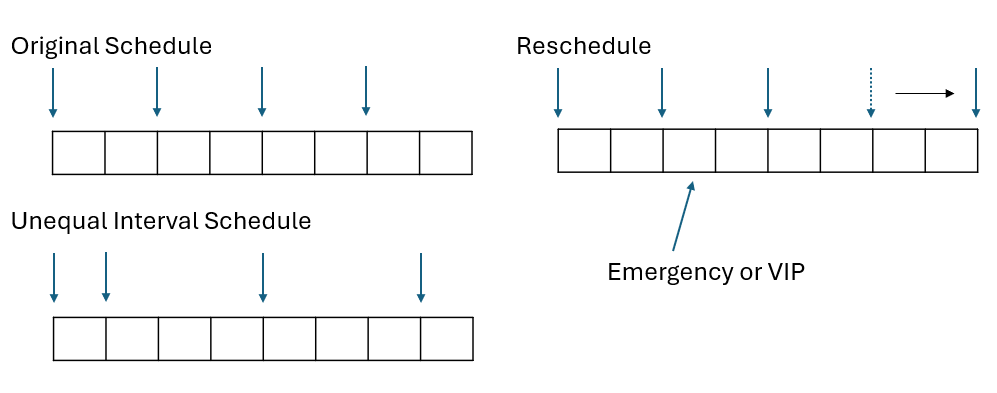
\includegraphics[width=0.7\textwidth]{./Figures/ex2.png}
\end{figure}
\end{example}

Innovation: Priority-based dynamic rescheduling with waiting capacity constraints

\section{Some instances}
We evaluate and compare three constraint scenarios: 

\begin{itemize}
    \item  Waiting Time Constraint: Limits the maximum waiting time for each customer.
    \item  Overlapping Time Constraint: Restricts simultaneous waiting overlaps.
    \item  Combined Constraints: Enforces both waiting time and overlapping time limits.
\end{itemize}

In all cases, the schedule times of later customers do not affect the appointments of preceding customers, ensuring feasibility in sequential scheduling.

Setting the mean of simultaneous waiting time to be no larger than zero (requiring that the number of people never exceeds a certain threshold) is an overly stringent condition. In systems without a maximum service time constraint, this requirement would significantly delay the scheduled time compared to systems that only consider the single waiting time. Moreover, when extreme situations occur (the service times of the earlier customers are extremely large), the scheduled time would be postponed even further.


% direction: put the overlapping time in objective function or put it in the constraint.
An alternative approach is to set a threshold on the probability of the number of waiting customers not exceeding a certain limit.


%   1. 学术研究中的考虑
%   群体等待时间的优化目标:部分研究会将总等待时间(total waiting time)或平均等待时间作为优化目标,这间接涉及多人共同等待的累积效应。例如:
  
%   在门诊调度中,最小化所有患者的等待时间总和。
%   在制造业中,减少批次任务的总延迟时间。
  
%   公平性约束:某些场景(如公共服务)会引入公平性指标,避免某些群体等待时间过长。例如:
  
%   限制不同优先级群体的最大等待时间差异。
%   使用加权调度算法平衡不同用户的等待体验。


% 2. 行业实践中的要求
% 显性限制较少:行业标准(如医疗、银行、客服中心)通常更关注个体等待时间的上限(如“95%的患者等待时间不超过30分钟”),而非多人共同等待的总和。

% 隐性管理需求:以下场景可能涉及群体等待的间接控制:

% 服务容量规划:通过计算峰值时段的平均等待时间,反推需增加的资源(如窗口、人员)。
% 动态调度:在机场安检、餐厅排队等场景中,系统会实时监测队列长度(即群体等待的直观体现),并动态调整资源。
% 批次处理(Batch Processing):如实验室检测、物流分拣,需权衡单个样本的等待时间与整体吞吐量。


% punctuality. congestion effect. pre-empt policy. walk-in. fairness. priority. patient preference.

The original model considers the single segment of the overlapping,


\begin{equation}\label{single_overlap}
    \begin{aligned}
        \min \quad & E[T_{n}(\Z_{n}, \D_{n-1})] \\
        \mbox{s.t.} \quad & E[W_{i,i+1}(\Z_{i-1}, \D_{i})] \leq w, i=2,\ldots, N-1
    \end{aligned}
\end{equation}

For this model, only the seperate overlapping period is considered. From the perspective of customer $i+1$, the total overlapping time can be calculated by $E[W_{i,i+1}(\Z_{i-1}, \D_{i})] + E[W_{i+1,i+2}(\Z_{i-1}, \D_{i})]$.


\begin{equation}\label{total_overlap}
    \begin{aligned}
        \min \quad & E[T_{n}(\Z_{n}, \D_{n-1})] \\
        \mbox{s.t.} \quad & E[W_{i-1,i}(\Z_{i-1}, \D_{i}) + W_{i,i+1}(\Z_{i}, \D_{i+1})] \leq w, i=2,\ldots, N-1
    \end{aligned}
\end{equation}



% 而对于 overlapping time model, 会对于某几个customer增加等待时间,但是控制了整体的传染风险。

% 对于N-2 个


\begin{table}[ht]
    \centering
    \caption{Schedule Intervals}
    \begin{tabular}{ccccccc}
    \hline
    \hline
    Waiting Model & $T_{n} = 188.76$ & $\Delta_1= 0.72$ & $\Delta_2= 31.1$ & $\Delta_3=31.3$ & $\Delta_4 = 32.3$ & $\Delta_5=32.5$ \\
    Waiting  &  0 & 30  & 30  & 30 & 30 & 30 \\
    Overlapping & 0 &  5.2 & 12.4 & 15.4 & 17.1 & 8.9 \\ 
    \hline
    Overlapping Model & $T_{n} = 189.13$ & $\Delta_1= 0.02$ & $\Delta_2= 30.0$ & $\Delta_3 = 29.6$ & $\Delta_4= 41.2$ & $\Delta_5 =27.2$ \\
    Waiting   & 0  & 30.7 & 31.7  & 33.2 & 26.6 & 30.3 \\
    Overlapping & 0 & 6.1 & 15  & 15 & 15 & 8.9 \\
    \hline
    Waiting Model & $T_{n} = 156.36$ & $\Delta_1= 0.72$ & $\Delta_2= 31.1$ & $\Delta_3=31.3$ & $\Delta_4 = 32.3$ \\
    Waiting  & 0 & 30  & 30  & 30 & 30 \\
    Overlapping & 0 &  5.2 & 12.4 & 15.4 & 8.2 \\ 
    \hline
    Overlapping Model & $T_{n} = 156.21$ & $\Delta_1= 0$ & $\Delta_2= 24.4$ & $\Delta_3 = 42.3$ & $\Delta_4= 26.2$ \\
    Waiting  &  0  & 30.8 & 37.1  & 27.7 & 32.4 \\
    Overlapping & 0 & 9.3 & 15  & 15  & 9.3 \\
    \hline
    \end{tabular}
  \end{table}

Several conclusion:

For the waiting time constraint model: the average individual waiting time remains stable, but the overlapping duration among individuals grows, leading to elevated transmission risk.

For the overlapping time model: while this model may marginally extend waiting times for a subset of customers, it effectively mitigates overall transmission risk by controlling concurrent waiting.



\end{document}
